\chapter{GroundOne: Method and Implementation}
\label{sec:method}

% Source notes: Project/docs/thesis_notes.md (Ch. 3), Project/docs/dataset_plan.md §8, implementation_plan.md §4.

GroundOne is a compact language model used as a decision model. It reads the document and the answer once and, without
generating text, returns a verdict for each scored sentence of the answer, deriving it from the logits of a few answer
letters. The chapter first describes the decision the model makes and the prompt that gathers all the decisions about
one answer into a single forward pass. It then presents the training objective, the calibration of the output
probabilities and the rule that turns the probabilities into the returned labels, and it closes with the software that
implements all of this.

\section{Task and decision}
\label{sec:method-task}

For every sentence of an answer, GroundOne chooses among three classes, defined in Section~\ref{sec:data-task}: with
respect to the document, the sentence is \emph{supported}, \emph{contradicted} or \emph{not mentioned}. The
\emph{document} is the whole context that the generator received. It may comprise several retrieved passages, possibly
from different sources, concatenated in the prompt: this is the case of question answering in RAGTruth
(Section~\ref{sec:data-sources}). A sentence is therefore supported when at least one passage backs it, including by
combining information scattered across different passages.

Each class
corresponds to a letter (A, B and C), and the model returns a probability for each of them. This is the only question
the model receives: everything else is derived from these three probabilities. The binary groundedness score is the
probability that the sentence is supported. The strict policy flags every unsupported sentence, while the lenient
policy flags only contradicted sentences. A single forward pass is therefore enough for all these uses.

Asking the model a separate question for each policy would add nothing: once the class of a sentence is known, how each
policy judges it is already known too. Separate questions would only multiply the number of decisions and, in
training, would risk teaching the model mutually inconsistent answers about the same sentence.

\section{All verdicts in a single forward pass}
\label{sec:method-readout}

The prompt contains a short instruction, the document and the answer. The sentences of the answer are numbered, and
every sentence associated with a decision is followed by a marker, that is, a short fixed string that indicates where
the verdict is read: the string ``\texttt{~Verdict:}''. Sentences without checkable content
(Section~\ref{sec:data-construction}) remain in the text as context, but without a marker. The model processes the
whole sequence once. At the last token of each marker the logits of the letters A, B and C are read and normalised
with a softmax\footnote{The \emph{softmax} turns a vector of scores into a probability distribution: each score $z_i$
becomes $e^{z_i} / \sum_j e^{z_j}$. Restricting it to three letters means computing it only over their three logits,
ignoring the rest of the vocabulary.} restricted to these three letters.
In a decoder each position sees only the preceding ones, so the verdict on sentence $i$ depends on the document and on
sentences $1, \dots, i$. This is exactly what verification needs, because references, such as pronouns, point
backwards. What follows the last marker affects no verdict, so the sequence ends there. Figure~\ref{fig:method-marked} shows the structure of the prompt and the points where the readout takes place.

\begin{figure}[htbp]
\centering
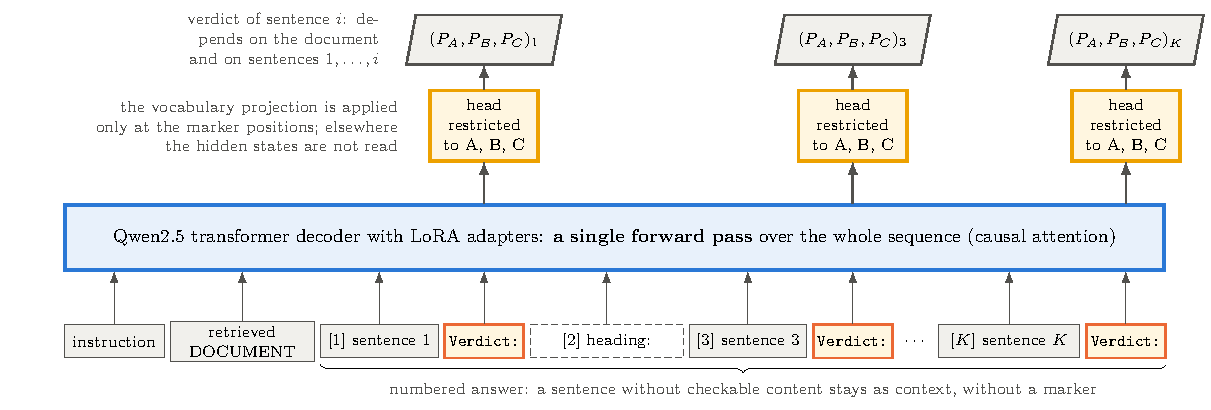
\includegraphics[width=\textwidth]{images/diagrams/method_marked_prompt_tikz.pdf}
\caption{The marker prompt of GroundOne (design b). The sentences of the answer are numbered and every scored sentence is followed by the marker ``\texttt{~Verdict:}''; a sentence without checkable content (here a heading) remains as context, without a marker. The model processes the whole sequence in a single forward pass, and the output head, restricted to the letters A, B and C, is applied only at the marker positions. Because of causal attention, the verdict on sentence $i$ depends on the document and on sentences 1 to $i$.}
\label{fig:method-marked}
\end{figure}

Two details make the readout exact and efficient. The first concerns exactness: the prompt is built by tokenising its
parts separately and then concatenating them, so that the position of every marker is known exactly and stays
identical in training and at inference. The second concerns efficiency: the output projection onto the vocabulary is
applied only at the marker positions. The transformer body processes the whole sequence, but the large vocabulary
matrix is multiplied only by the few hidden states that are actually read, that is, by the vectors the model computes
at the marker positions.

The marker readout also determines the cost of a verification. Let $S$ denote the total length of document and answer,
$K$ the number of decisions and $m$ the length of a marker in tokens. The decision model requires a single prefill of
$S + K m$ tokens. A generative judge, in contrast, must also produce its verdicts during decoding. If each verdict
requires $n$ tokens and each decoded token takes a time $t_\mathrm{dec}$, the cost of the judge is roughly
$\mathrm{prefill}(S) + K\, n\, t_\mathrm{dec}$. A marker is only three tokens long, whereas on the reference hardware
decoding is much slower than prefill for the same number of tokens; the gap between the two costs therefore widens as
$K$ grows. On the M4 used in this thesis, with the 0.5B model prefill costs about 0.37\,ms per token and decoding
5.9\,ms per generated token; with the 3B the two values are 2.2 and 31.8\,ms. One decoded token thus costs as much as
fourteen to sixteen tokens in prefill. The two phases also stress the hardware differently. Prefill processes many
tokens together and is limited by compute, whereas decoding produces one token at a time and is limited by the
bandwidth needed to read the weights~\cite{pope2023scaling,patel2024splitwise}. The difference resurfaces in the
energy measurements of Chapter~\ref{sec:results}. Figure~\ref{fig:method-cost} translates the cost model into seconds per answer, using only these measured constants.

\begin{figure}[htbp]
\centering
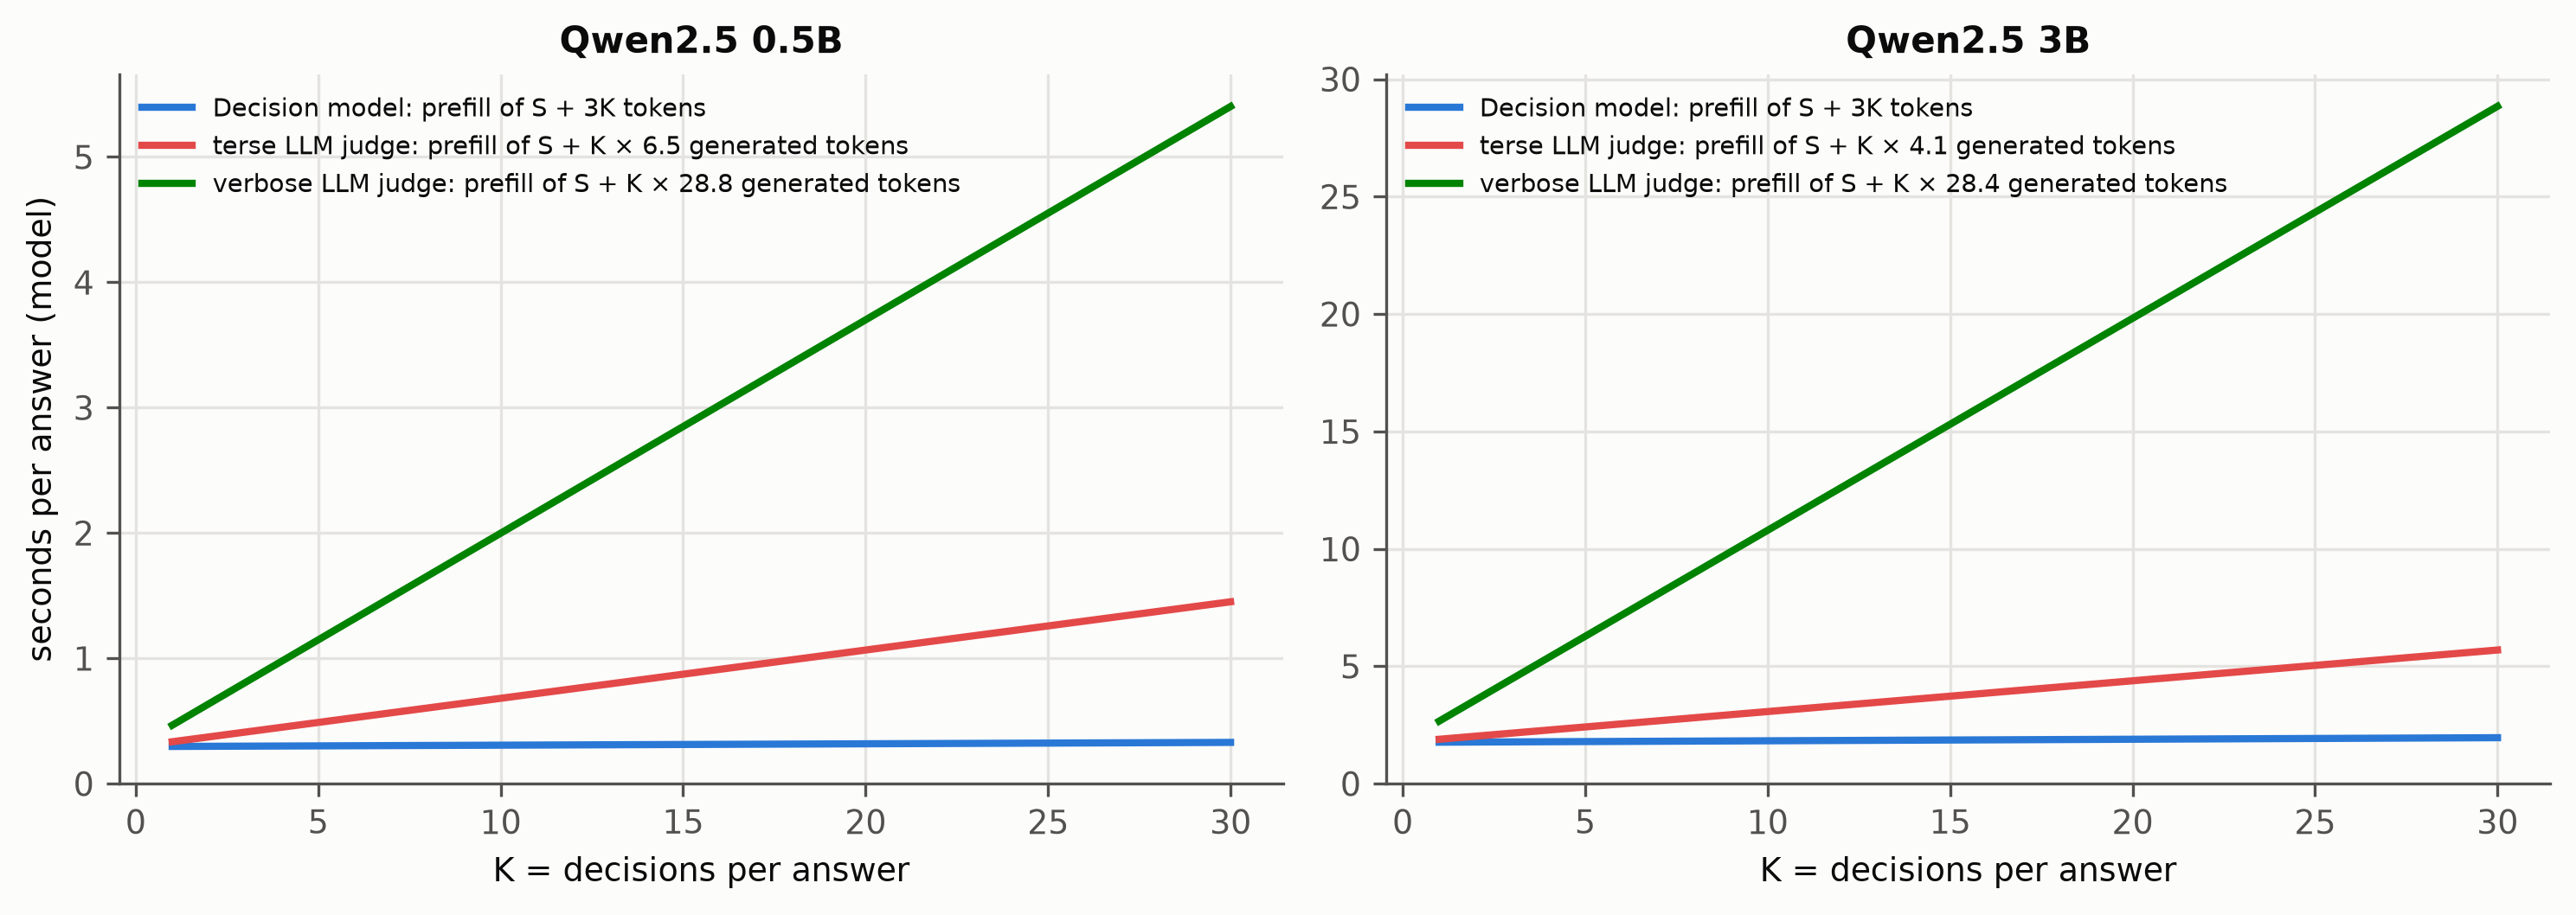
\includegraphics[width=\textwidth]{images/method/cost_model.png}
\caption{Estimated cost of verifying an answer of $S = 800$ tokens as a function of $K$, computed with only the constants measured on the M4: the per-token time of prefill and decoding and the mean number of tokens each judge generates per verdict on the latency subset (mean $K$ 8.7). It is an analytical model, not a measurement: the measured latencies are in Section~\ref{sec:results-latency}. The cost of the decision model grows by only three prefill tokens per decision, that of the judges by a few decoding tokens per decision.}
\label{fig:method-cost}
\end{figure}

There is also a second solution, which reads the shared prefix once and then appends a short question for each
sentence, evaluating the questions in a batch. Unlike the marker solution, which needs only a single forward pass, this
one requires a KV cache replicated $K$ times. It is kept as a fallback and is the natural format for an untrained
model, which understands an explicit question but has no reason to interpret a marker as a request for a verdict. For
this reason it is the format used by the untrained baseline (Section~\ref{sec:setup-baselines}).
Figure~\ref{fig:method-designs} compares the two solutions.

\begin{figure}[htbp]
\centering
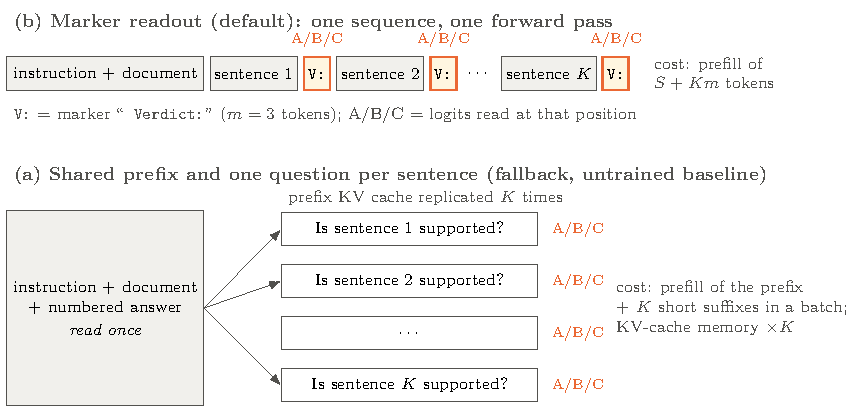
\includegraphics[width=\textwidth]{images/diagrams/method_designs_ab_tikz.pdf}
\caption{The two solutions for obtaining $K$ verdicts from a single reading. (b) The marker readout, adopted as the default, inserts a marker after every sentence and reads all the verdicts in the same pass. (a) The fallback solution reads the shared prefix once and appends a short question for each sentence, evaluated in a batch; it requires, however, $K$ copies of the KV cache of the prefix, and it is the natural format for an untrained model.}
\label{fig:method-designs}
\end{figure}

\paragraph{A classifier, not a faster generator.} The readout restricts the decision to three letters, and the
restriction is not a detail. After the marker, the fine-tuned model would not write the letter that is read. Its most
probable next token is in fact the same letter preceded by a space, which for the tokenizer is a different token. At the
markers, the three readout letters together collect only about 4--5\,\% of the probability mass. A loss restricted to
these letters trains their relative logits, not their absolute probability, and the readout therefore behaves as a
three-class classifier grafted onto the language model. This is what defines a decision model: the answer never goes
through decoding, but is chosen among the admissible options.
The phenomenon also recalls two results from the literature: the probability of the first answer token and the answer
the model actually writes may not coincide~\cite{wang2024myanswerc}, and the choice among letters is subject to
selection bias~\cite{zheng2024mcq}. A specialised, calibrated readout has to absorb both effects. A control experiment
quantifies its difference from generation: it keeps the same weights and the same forward pass, but instead of the
restricted readout it takes the token that generation would emit (Section~\ref{sec:results-readout}).

% Marker " Verdict:" = 3 tokens with the Qwen2.5 tokenizer (" Ver", "dict", ":"), verified 2026-10-07.
% Prefill / decode speeds: Phase 0 measurements (Project/docs/phase0_report.md). Readout mass: thesis_notes.md (B2 check).

\section{Training objective}
\label{sec:method-training}

GroundOne is obtained from Qwen2.5-0.5B-Instruct and Qwen2.5-3B-Instruct~\cite{qwen2024qwen25} through low-rank
adaptation (LoRA)~\cite{hu2022lora}, described in Section~\ref{sec:bg-peft} (Figure~\ref{fig:bg-lora}). The adapters have rank 16, scaling factor 2 and dropout 0.05\footnote{The \emph{scaling
factor} multiplies the update computed by the adapter before it is added to the output of the frozen layer.
\emph{Dropout} randomly zeroes, during training, a fraction of the adapter's inputs (here 5\,\%), so as to reduce the
risk that the model memorises the training set.}. They are applied to all the linear layers of all the transformer
blocks, that is, to the seven projections of each block (Figure~\ref{fig:method-lora}), because covering every layer
matters more than using a high rank~\cite{dettmers2023qlora}. In total, 8.8 million parameters are trained in the 0.5B
and 29.9 million in the 3B, about 1.8\,\% and 1.0\,\% of the respective models. The weights of the base model
remain frozen at 8-bit precision. Each training example is an answer with all its scored sentences, and the loss is
computed at each of its markers.

\begin{figure}[htbp]
\centering
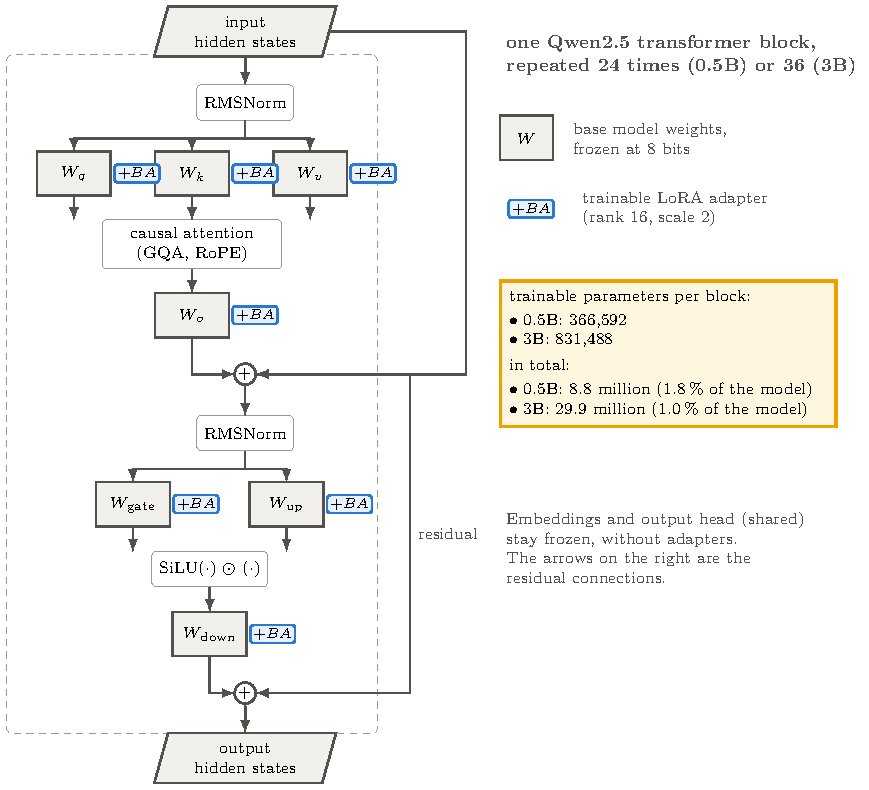
\includegraphics[width=0.95\textwidth]{images/diagrams/method_lora_placement_tikz.pdf}
\caption{Where GroundOne applies LoRA. Each transformer block of Qwen2.5 contains seven linear projections: four
in the attention ($W_q$, $W_k$, $W_v$, $W_o$) and three in the MLP block ($W_\mathrm{gate}$, $W_\mathrm{up}$, $W_\mathrm{down}$).
Their weights remain frozen at 8 bits, and each is paired with a rank-16 adapter (in blue) that corrects its
output following the scheme of Figure~\ref{fig:bg-lora}. The block is repeated 24 times in the 0.5B and 36 in the 3B;
the embedding and the output head have no adapter.}
\label{fig:method-lora}
\end{figure}

The loss is a cross-entropy\footnote{The \emph{cross-entropy} of a prediction is the negative logarithm of the
probability the model assigns to the correct class: it is zero when this probability is one and grows without bound
when the model is confidently wrong.} computed over the three letters only. The prompt is never supervised, so the
training signal comes entirely from the verdicts. About 88\,\% of the sentences in the training set are supported, so
the classes are weighted so that each contributes equally to the loss. With the distribution of the training set this
gives weights of about 0.38 for supported sentences, 7.5 for contradicted ones and 4.4 for not-mentioned ones. Without
these weights, a model can reach a low loss by answering ``supported'' almost always. A useful consequence follows: a
model that had learnt only the class frequencies would remain at a loss of $\ln 3 \approx 1.10$, so a loss below this
value indicates that the model actually exploits the text.

The optimiser is AdamW, used without weight decay, that is, without the penalty that shrinks the magnitude of the
weights at every step. As in the default configuration of MLX, the moment estimates receive no bias correction, and no
gradient clipping is applied. Training lasts one epoch, that is, a single pass over the answers of the training set.
The learning rate rises to $10^{-4}$ with a linear warm-up over the first 3\,\% of the steps and then decreases to zero
with a cosine schedule\footnote{During the \emph{warm-up} the learning rate grows gradually to the chosen value, so as
to avoid abrupt updates at the start of training. The \emph{cosine schedule} then reduces it following half a period of
a cosine: slowly at first, faster in the middle and slowly again towards the end.}. Answers of similar length are
grouped into micro-batches, each within a token budget that also includes padding, that is, the filler tokens that
equalise the lengths. The gradients of several micro-batches are then accumulated, so that each optimiser step sees
about 16 answers, or about 110 decisions. In this way every step contains some contradicted sentences, despite the
rarity of the class. Gradient checkpointing, which recomputes some activations during the gradient computation instead
of storing them, keeps memory usage within the 16\,GB of the laptop.
During training the model is evaluated periodically on the dev set, and the checkpoint, that is, the copy of the
weights, with the highest three-class balanced accuracy, averaged over the three tasks of RAGTruth (question answering, summarisation and data-to-text), is kept. Section~\ref{sec:setup-models} reports
the settings of each run.

\section{Calibration}
\label{sec:method-calibration}

The class weights train the model as if the three classes were equally frequent, so its raw probabilities do not
reflect the real class frequencies. A post-hoc transformation is therefore fitted on the dev set and applied to the
logits after training, without changing the weights. The three logits are divided by a temperature $T$ and shifted by
a per-class bias, $\mathrm{softmax}(z / T + b)$, with the bias of the supported class fixed at zero. The parameters $T$
and $b$ are chosen by minimising the negative log-likelihood (NLL) of the dev-set
labels\footnote{The \emph{negative log-likelihood} of a set of $n$ predictions is the mean, with the sign changed, of the logarithm of the probability assigned to the correct class: $\mathrm{NLL} = -\frac{1}{n}\sum_{i=1}^{n} \log p_i(y_i)$, where $y_i$ is the correct class of prediction $i$. It coincides with the mean cross-entropy. It is zero when the model always assigns probability one to the right class and grows rapidly when it assigns a low probability to the right class, that is, when it is confidently wrong: this is why it penalises both errors and overconfidence.}, that is, the mean cross-entropy~\cite{guo2017calibration}. The bias plays the role of the contextual calibration proposed for
language models queried through prompts~\cite{zhao2021calibrate}; unlike that correction, however, here it is fitted
on labelled data. Temperature alone changes the probabilities but neither the most probable class nor the ranking of
the sentences. The bias, instead, can change the most probable class and, with three classes, can also slightly
reorder $P(\text{supported})$ from one sentence to another. For this reason the classification metrics and the
AUROC\footnote{The \emph{AUROC} (area under the ROC curve) measures how well a score separates two classes, here
supported from unsupported sentences. Given a threshold, the sentences with a higher score are accepted as supported:
the share of supported sentences accepted is the true positive rate, the share of unsupported sentences accepted by
mistake is the false positive rate. The ROC curve plots these two quantities for all possible thresholds, and the
AUROC is the area under it. It equals the probability that a randomly chosen supported sentence receives a higher
score than a randomly chosen unsupported sentence: it is 0.5 for a random score and 1 for perfect separation.} are
computed on the raw output. The calibrated probabilities are used instead wherever a probability has to correspond to
a frequency: in the calibration metrics, in the thresholds and in selective prediction
(Section~\ref{sec:results-calibration}).

\paragraph{Calibration during or after training.} GroundOne calibrates its probabilities after training. Jev, the
decision model that introduced the category, takes the opposite route: according to the vendor, its probabilities
become reliable already during training, thanks to a reinforcement learning phase with rewards designed to reward
calibration (\emph{Reinforcement Learning with Calibrated Decisions}, RLCD)~\cite{typesafe2026jev}. The recipe is not
public, and a direct comparison was not possible: Jev is a remote, closed service, and evaluating it on the test sets
of this thesis would have required sending the data to an external service. The comparison therefore concerns the
approaches, on the basis of the independent evaluations (Table~\ref{tab:method-calibration-jev}).

These evaluations show that calibration obtained during training holds in aggregate, but not on the individual
workload. Over 31 benchmarks the ECE of Jev is 0.047 when computed on all the data together, but 0.168 as the median of
the individual benchmarks~\cite{guo2026justaskjev}. Its binary probabilities rank the examples well, but they are
slightly underconfident, so the fixed threshold of 0.5 ends up poorly placed: the mean probability of an affirmative
answer is 0.465, against an observed frequency of 0.518~\cite{deusser2026jev}. For this reason the studies recommend
fitting thresholds and temperatures on the target workload~\cite{li2026jevjudge}. Even the openly released RLCD recipe
offers no measurable advantage: in a controlled comparison it remains 2.5 to 3 points below plain cross-entropy, with a
variability across seeds up to four times larger, and after temperature scaling no training objective turns out to be
better calibrated than the others~\cite{deka2026typed}.

GroundOne starts from here. A specialist works on a single domain, so it can fit its own calibration on exactly the
distribution in which it will be used, with a dev set and a few parameters. On T1 the binary ECE falls from 0.30 to
0.019 for the 0.5B and from 0.18 to 0.019 for the 3B. The price is the same one that the studies find for Jev, seen
from the other side: the calibration fitted on RAGTruth does not transfer to VitaminC
(Section~\ref{sec:results-calibration}). The advantage is that the procedure is open, reproducible and bound to the
model that produced it, and that the decision threshold is part of the calibration instead of being left to the user.

\begin{table}[htbp]
\centering
\caption{Two approaches to the calibration of a decision model. The values for Jev come from independent evaluations
on benchmarks different from those of this thesis; those for GroundOne are measured on the T1 test set.}
\label{tab:method-calibration-jev}
\small
\begin{tabular}{p{0.19\textwidth}p{0.35\textwidth}p{0.35\textwidth}}
\toprule
 & Jev & GroundOne \\
\midrule
When & During training: SFT followed by RL with calibration rewards (RLCD). & After training: temperature and per-class bias fitted on the dev set. \\ \addlinespace
Scope & A single model for all tasks. & A single domain, the one in which the model is used. \\ \addlinespace
Recipe & Not public (vendor's statement). & Open and bound to the model fingerprint. \\ \addlinespace
Threshold & Left to the user; it must be fitted for each workload. & Fitted on the dev set and part of the output rule. \\ \addlinespace
Evidence & ECE of 0.047 in aggregate and 0.168 per individual benchmark; underconfident binary probabilities. & Binary ECE on T1 from 0.30 to 0.019 (0.5B) and from 0.18 to 0.019 (3B); does not transfer to VitaminC. \\
\bottomrule
\end{tabular}
\end{table}

Calibration is measured mainly with the Expected Calibration Error
(ECE)~\cite{naeini2015ece,guo2017calibration}, which measures how far, on average, the confidence stated by a model
departs from the frequency with which its predictions turn out to be correct. The $n$ predictions are divided, according
to their confidence, into $M$ intervals of equal width, with $M = 15$ in this thesis. For each interval $B_m$ the mean
confidence of its predictions, $\mathrm{conf}(B_m)$, is compared with the fraction of them that turned out to be
correct, $\mathrm{acc}(B_m)$. The ECE is the mean of the gaps, weighted by the size of the intervals:
\begin{equation}
  \mathrm{ECE} = \sum_{m=1}^{M} \frac{|B_m|}{n} \, \bigl| \mathrm{acc}(B_m) - \mathrm{conf}(B_m) \bigr| .
  \label{eq:ece}
\end{equation}
A perfectly calibrated model has an ECE of zero; an ECE of 0.05, for example, indicates that the stated confidence
departs on average by five percentage points from the observed frequency. In the binary variant the confidence is $P(\text{supported})$ and the
observed frequency is the share of supported sentences in the interval. In the three-class top-label variant, instead,
the confidence is the maximum probability and the observed frequency is the share of correct predictions. The ECE does
not compare the distribution of the predicted classes with that of the test set. Rather, it checks whether, among the
sentences to which the model assigns a given confidence, that confidence matches reality. The measure has two limits,
however: it depends on the choice of intervals, and a constant predictor that always returns the base rate obtains an
ECE close to zero while discriminating nothing. For these reasons the ECE is always reported together with the Brier
score\footnote{The \emph{Brier score} is the mean squared error between the predicted probability and the observed
outcome, coded as 1 if the event occurs and 0 otherwise: the lower it is, the better the probabilities.}, the negative
log-likelihood and reliability diagrams, the plots that show, for each interval, the observed frequency as a function
of the mean confidence. The ability of the probabilities to separate correct from wrong decisions is measured
separately instead, with two measures. The first is the AUROC, described below. The second is the AURC (area under the
risk--coverage curve), that is, the area under the risk--coverage curve of Section~\ref{sec:bg-calibration}
(Figure~\ref{fig:bg-risk-coverage}): it measures the mean error rate obtained by accepting the decisions from the most
to the least confident, and it is smaller the more the errors are concentrated among the least confident decisions,
which are those a system would defer.

Calibration and AUROC answer two different questions, which is why the thesis always reports both. The ECE asks
whether a probability of 0.8 really corresponds to a sentence that is supported eight times out of ten. The AUROC asks
instead whether supported sentences receive higher scores than unsupported ones, whatever the scale of the scores
(Figure~\ref{fig:method-roc}). The two properties are independent. A constant predictor is perfectly calibrated with
respect to the base rate, but has an AUROC of 0.5; conversely, a model can rank the sentences almost perfectly, with an
AUROC close to 1, and still assign overly extreme probabilities. The AUROC, moreover, depends neither on any threshold
nor on the class frequencies, and it does not change if the scores are transformed monotonically, as temperature does.
For this reason it is the main measure by which GroundOne is compared with verifiers that return a binary score, such
as the specialised encoders, while the choice of the threshold and its consistency with the probabilities shown to the
user are treated separately.

\begin{figure}[htbp]
\centering
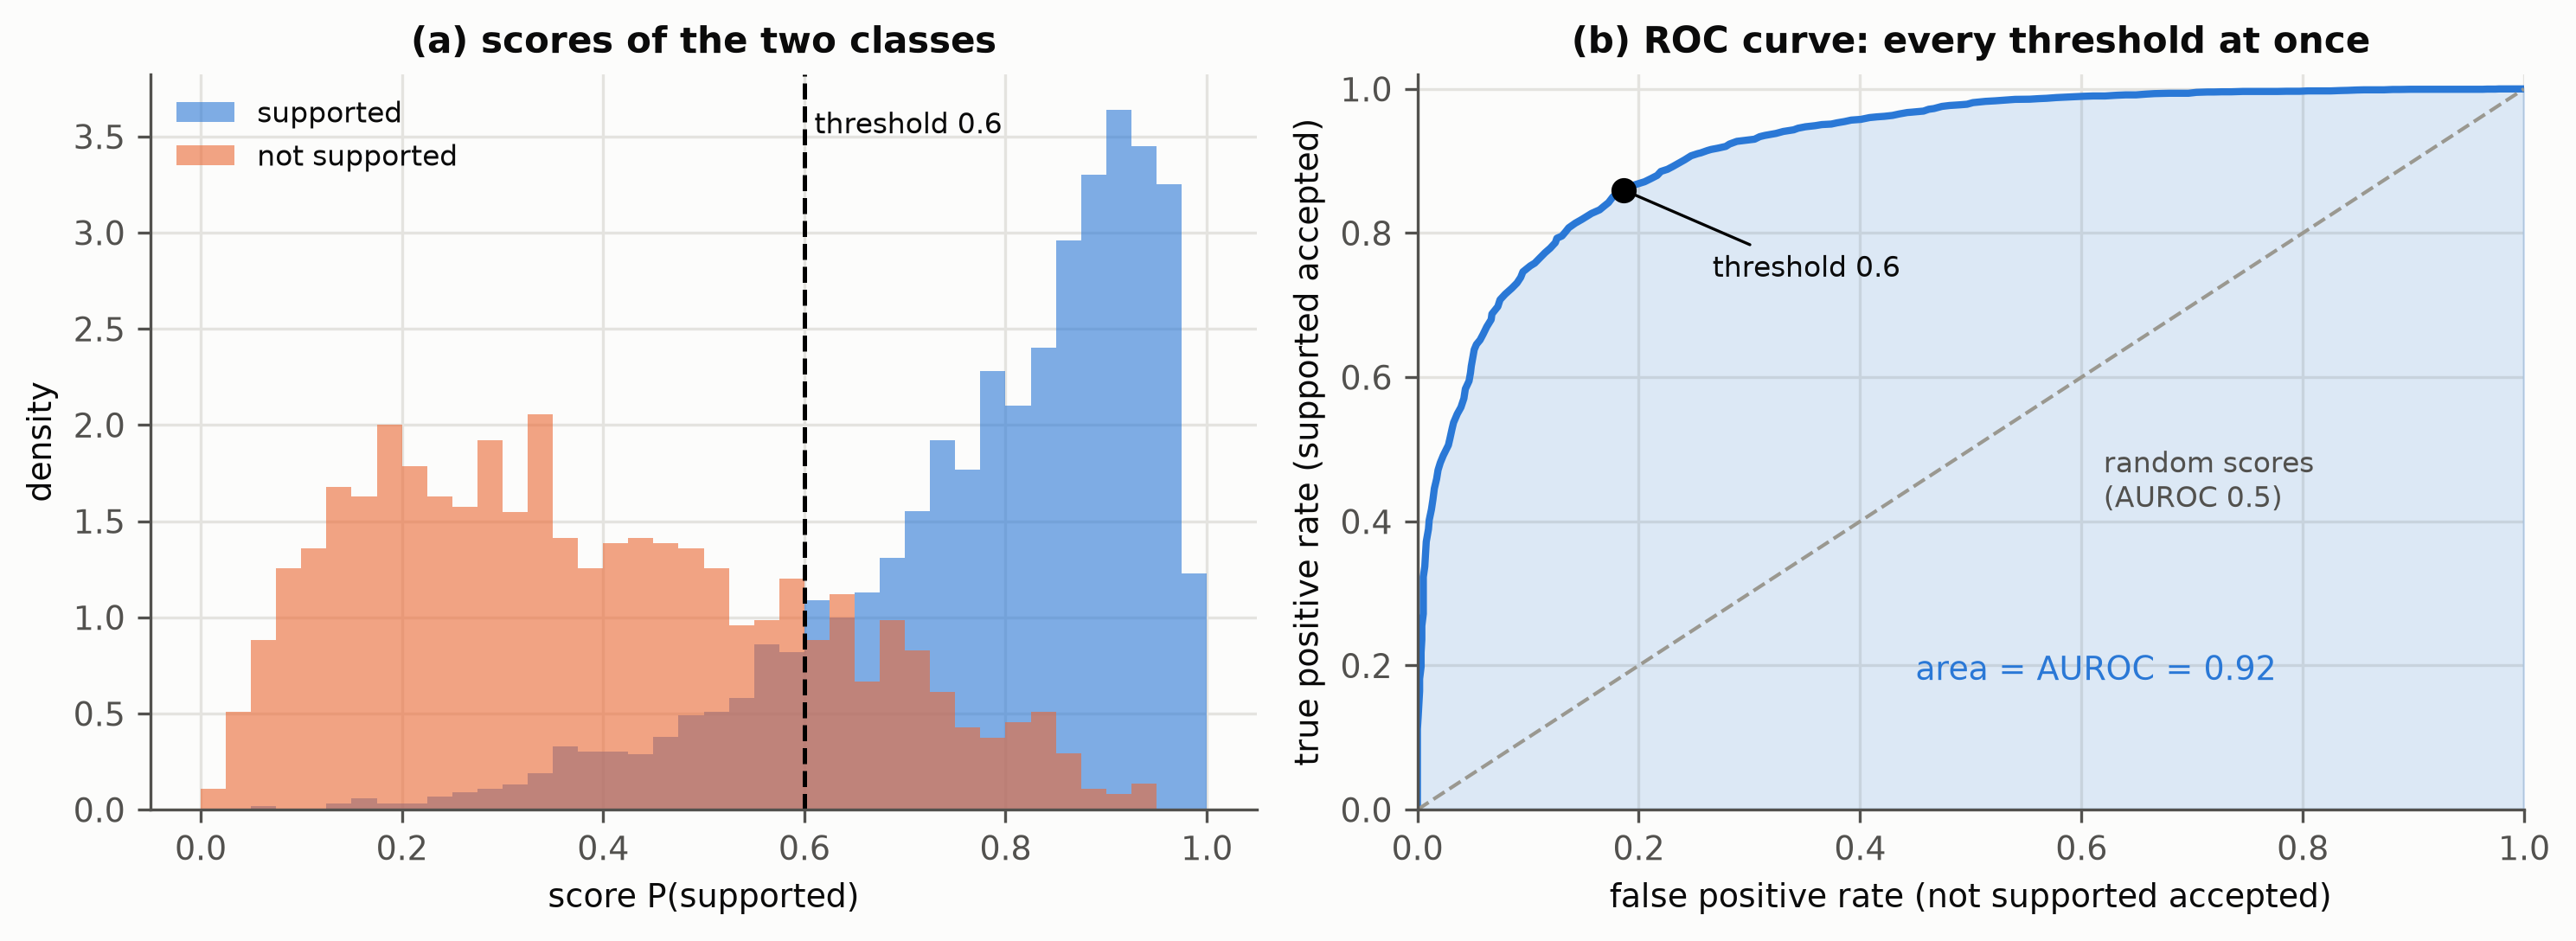
\includegraphics[width=\textwidth]{images/method/roc_explainer.png}
\caption{How the AUROC arises (a sketch with synthetic scores, not a result). (a) Distribution of $P(\text{supported})$
for supported and unsupported sentences: the two distributions overlap, and every threshold accepts part of each.
(b) Moving the threshold from 1 to 0 yields the ROC curve; the black dot corresponds to the threshold of
panel (a). The area under the curve is the AUROC: the more separated the two distributions, the closer the curve gets
to the top-left corner and the area to 1. The diagonal corresponds to random scores.}
\label{fig:method-roc}
\end{figure}

\paragraph{From probabilities to returned labels.} A user of the verifier sees, for each sentence, a label and a
probability, which must be consistent with each other. This thesis evaluates the raw decision, that is, the most
probable class according to the uncalibrated output. The raw decision, however, can contradict the calibrated
probability shown next to it: a sentence can be labelled ``not mentioned'' while having a calibrated
$P(\text{supported})$ slightly above one half. The returned output therefore derives every element from the calibrated
probabilities with a single rule. A sentence is labelled supported if and only if $P(\text{supported}) \geq \tau$;
otherwise it receives the more probable of the two remaining classes. The strict policy flags every unsupported
sentence, the lenient one only contradicted sentences. The threshold $\tau$ is fitted on the dev set so as to maximise
the three-class balanced accuracy. The user can change it in every request, thereby choosing a different operating
point without retraining the model. Figure~\ref{fig:method-calflow} summarises the path from the raw logits to the returned labels.

\begin{figure}[htbp]
\centering
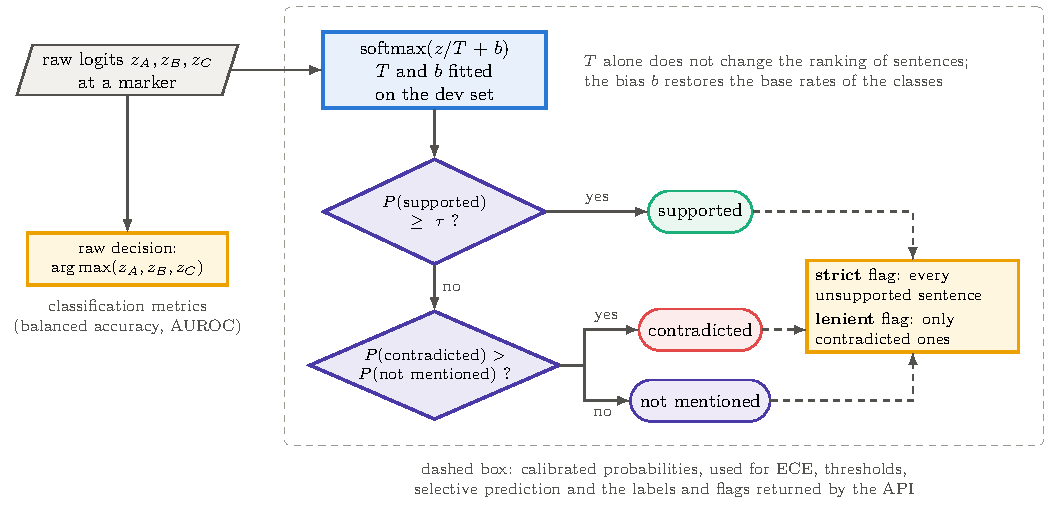
\includegraphics[width=\textwidth]{images/diagrams/method_calibration_flow_tikz.pdf}
\caption{From logits to returned labels. The raw decision, that is, the argmax of the logits, serves the classification metrics of Chapter~\ref{sec:results}. The calibrated probabilities, obtained with temperature and bias fitted on the dev set, feed instead the single rule of the returned output: supported if $P(\text{supported}) \geq \tau$, otherwise the more probable of contradicted and not mentioned. The strict and lenient flags derive from this.}
\label{fig:method-calflow}
\end{figure}

\section{Software}
\label{sec:method-software}

GroundOne is implemented as an installable Python package based on MLX~\cite{mlx2023,mlxlm}, the array framework
designed for Apple silicon. All the training and inference phases described so far run with MLX on the same laptop.
The package comprises the dataset builder with its checks, the training loop, calibration, evaluation on the frozen
test sets, the baselines and a memory-protection mechanism. The latter runs long processes one at a time and stops a
process before the system runs out of memory.

The verifier is exposed through a command-line interface and an HTTP server. The server offers a native endpoint and
an endpoint compatible with the System One interface of Jev, already used by other decision models, so that existing
clients can adopt GroundOne by changing only the address. The native endpoint receives a document and an answer. It
segments the answer with the same rule used to build the data and runs the single forward pass of
Section~\ref{sec:method-readout}. For each sentence it reports whether it was scored, the three calibrated
probabilities, the returned label and the flags of the strict and lenient policies, together with the decision rule
and the threshold that produced them. It also reports the number of input tokens, the number of generated tokens,
always zero, and the time taken. The compatible endpoint, instead, answers generic closed questions about a shared
context, with the one-question-per-sentence format. All the model computation takes place on a single long-lived
worker thread, because the Metal context of the GPU, that is, the state through which the program uses it via Apple's
graphics API, must not move from one thread to another. Finally, nothing leaves the machine: models, data and requests
stay local. Figure~\ref{fig:method-software} summarises the architecture of the package.

\begin{figure}[htbp]
\centering
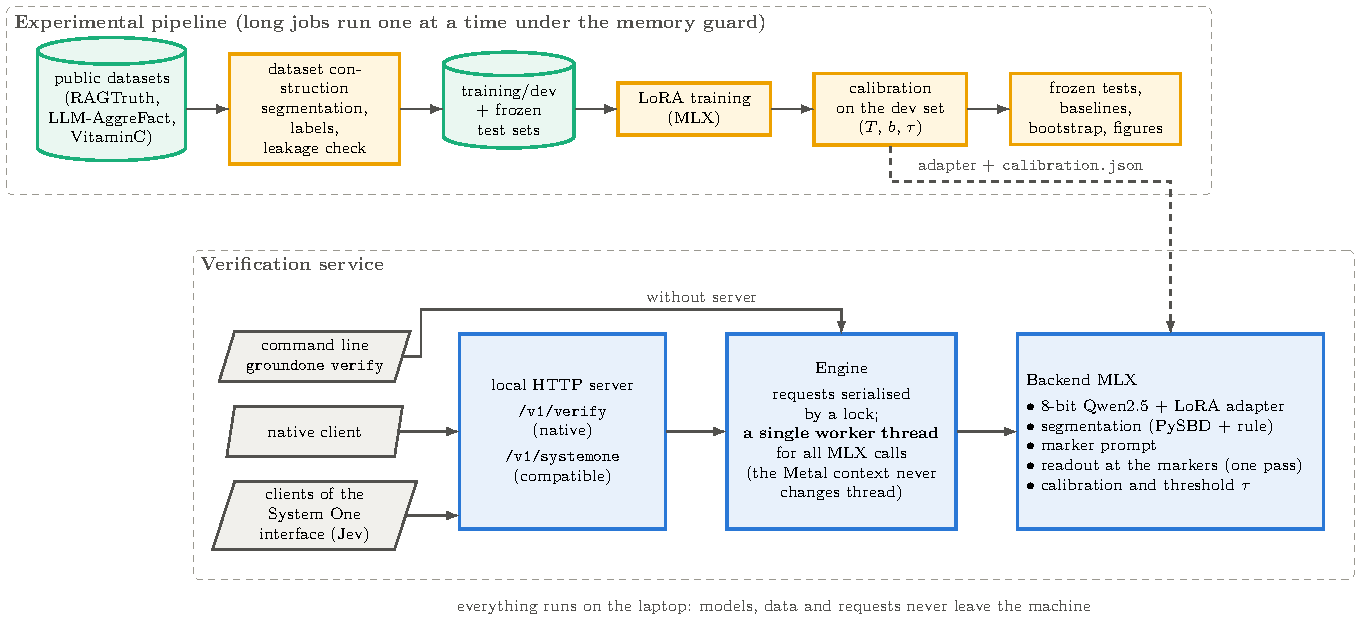
\includegraphics[width=\textwidth]{images/diagrams/method_software_tikz.pdf}
\caption{Architecture of the software. At the top, the experimental pipeline, from the public datasets to the frozen tests, run under the memory guard; at the bottom, the verification service, in which the command line and the HTTP server (native and compatible endpoints) share the same Engine, which serialises the requests and runs every MLX call on a single worker thread. The adapter and the calibration file produced by the pipeline are the only artefacts the service reads.}
\label{fig:method-software}
\end{figure}
